
Máquinas síncronas são aquelas em que existe dependência direta entre o número de rotações e a frequência das fontes geradas (no caso do alternador) ou entre a frequência da linha de alimentação e o número de rotações do rotor (caso do motor síncrono).

Uma máquina síncrona pode atuar como alternador ou como motor síncrono. Uma máquina síncrona como alternador tem como princípio de funcionamento os fenômenos de indução eletromagnética aos quais está sujeito um condutor ou uma espira sob variação de fluxo magnético. A variação de fluxo aparente para o condutor pode ser atingida fixando o campo indutor e movimentando (rodando) a espira ou fixando a espira e movimentando o campo.

\begin{figure}[ht!]
\center 
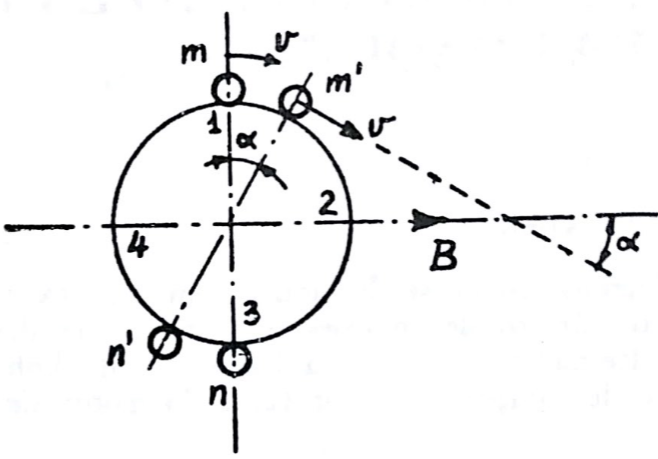
\includegraphics[scale=0.7]{imagens/1.png}
\caption{Espira "M" "N" em um campo magnético indutor.}\label{fig:1}
\end{figure}

Tomando como referência o esquema apresentado na figura \ref{fig:1}, vemos que a f.e.m $E_{M}$ adquire sentido positivo quando a espira está na posição (2-4), isto é, com o condutor $m$ no ponto 2 e o $n$ no ponto 4. O valor negativo verifica-se com a espira na posição (4-2). Ao passar pelo ponto (1-3) e (3-1) o valor de f.e.m é zero. 

\begin{figure}[ht!]
\center 
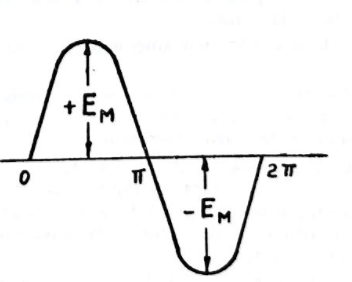
\includegraphics[scale=1]{imagens/2.png}
\caption{variação da f.e.m numa rotação completa da espira.}\label{fig:2}
\end{figure}

A partir desse sistema é possível perceber que a f.e.m varia em um período a cada rotação do induzido. Por essa razão, a frequência de rotação do induzido deve ser igual à frequência que se deseja obter.

Em um indutor de 4 polos (tetrapolar), como na figura \ref{fig:3}, por exemplo, a f.e.m induzida na espira completa um ciclo a cada meia rotação, uma vez que em meia rotação cada condutor da espira percorre um polo magnético norte e um polo sul. Dessa forma, numa rotação completa da espira, cada indutor seu percorre 2 polos norte e 2 polos sul.

\begin{figure}[ht!]
\center 
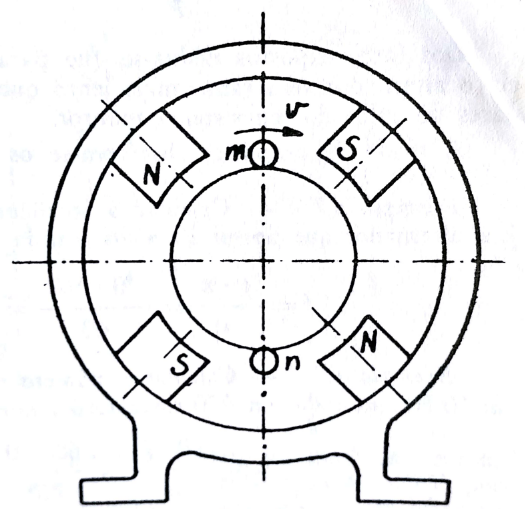
\includegraphics[scale=0.4]{imagens/3.png}
\caption{Indutor tetrapolar.}\label{fig:3}
\end{figure}

Vê-se que para $x$ pares de polos no alternador, para que as f.e.m geradas possuam a frequência $f$, é necessário que o induzido rode com $$n = \frac{f}{x}$$ rotações por segundo.

Portanto, caso desejássemos a velocidade de rotação do alternador em RPM, a fórmula ficaria $$n = {60}\frac{f}{x}$$.

A máquina elétrica possui a parte fixa (estator) e a parte girante (rotor), como ilustra a figura \ref{fig:4}.

\begin{figure}[ht!]
\center 
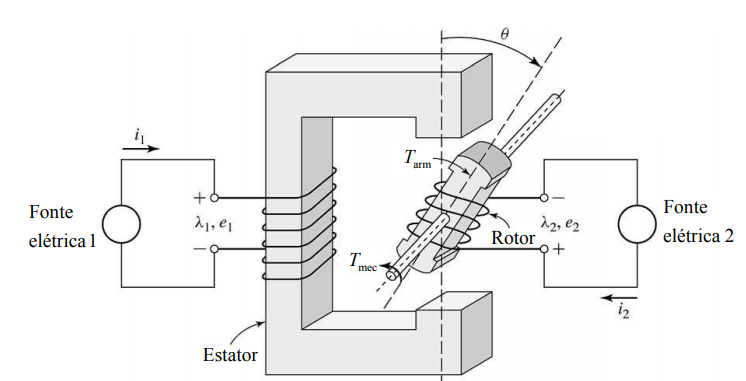
\includegraphics[scale=0.4]{imagens/4.PNG}
\caption{Estrutura da máquina.}\label{fig:4}
\end{figure}

O rotor está montado sobre o eixo e é livre para girar entre os polos do estator. De forma geral existem enrolamentos transportando corrente elétrica tanto no estator como no rotor.

A máquina síncrona pode funcionar tanto como gerador quanto como motor. Quando a
máquina síncrona funciona como gerador, energia mecânica é aplicada ao eixo da máquina, dando origem ao movimento de rotação. Dessa forma, o campo magnético que atravessa as bobinas do estator varia de forma senoidal, na frequência de rotação do rotor, induzindo tensões alternadas senoidais nos enrolamentos de armadura. A tensão induzida em cada enrolamento é dada pela equação:

$$E_f = 4,44  {f}\theta_f {N}{K_{w}}$$

Onde $E_f$ é a tensão eficaz por fase, $\theta_f$ é o fluxo do polo, $N$ o número de espiras do enrolamento e $K_w$ o fator de enrolamento. Para a maioria das máquinas trifásicas esse fator varia de 0,85 a 0,95.

Aparentemente, o produto entre a tensão e a corrente seria a potência necessária para o
motor executar o seu trabalho. Mas ocorre que, para o motor elétrico executar a transformação de energia elétrica em mecânica, ele necessita magnetizar os circuitos magnéticos do rotor e do estator. Desta forma, este produto entre a tensão e a corrente engloba dois componentes distintos de potência: 
\begin{itemize}
\item Um relacionado ao trabalho mecânico e perdas; e
\item Um para assegurar a existência dos campos magnéticos.
\end{itemize}

A potência aparente é definida como o produto entre a tensão e a corrente que é fornecida ao motor elétrico e é expressa em volt-ampère (VA). Para circuitos monofásicos é dada pela equação:

$$S = VI$$

E para circuitos trifásicos:

$$S = \sqrt{3}{VI}$$

A potência reativa é definida como a parcela de potência associada à magnetização dos
circuitos magnéticos e é expressa em volt-ampère reativo (VAr). Para circuitos monofásicos, é dada pela equação:

$$Q = VI \sin{\theta}$$

Para trifásicos:

$$Q = \sqrt{3}{VI} \sin{\theta}$$

A potência ativa é definida como a parcela de potência que o motor realmente converte em
energia mecânica, utilizada para acionar a carga, associada às perdas internas. Para circuitos monofásicos é dada pela equação:

$$P = VI \cos{\theta}$$

Para trifásicos:

$$P = \sqrt{3} VI \cos{\theta}$$

